%%% License: Creative Commons Attribution Share Alike 4.0 (see https://creativecommons.org/licenses/by-sa/4.0/)

\documentclass[english,10pt
,aspectratio=169
%,handout
%,notes
]{beamer}
%%% License: Creative Commons Attribution Share Alike 4.0 (see https://creativecommons.org/licenses/by-sa/4.0/)

\DeclareGraphicsExtensions{.eps, .pdf,.png,.jpg,.mps,}
\usetheme{reMedian}
\usepackage{parskip}
\makeatother

\renewcommand{\baselinestretch}{1.1} 

\usepackage{amsmath, amssymb, amsfonts, amsthm}
\usepackage{enumerate}
%\usepackage{enumitem}
\usepackage{hyperref}
\usepackage{url}
\usepackage{bbm}
\usepackage{color}

\usepackage{tikz}
\usepackage{tikzscale}
\newcommand*\circled[1]{\tikz[baseline=(char.base)]{
		\node[shape=circle,draw, inner sep=-20pt] (char) {#1};}}
\usetikzlibrary{automata,positioning}
\usetikzlibrary{decorations.pathreplacing}
\usepackage{pgfplots}
\usepgfplotslibrary{fillbetween}
\usepackage{graphicx}

\usepackage{setspace}
\thinmuskip=1mu
\medmuskip=1mu 
\thickmuskip=1mu 


\usecolortheme{default}
\usepackage{verbatim}
\usepackage[normalem]{ulem}

\usepackage{apptools}
\AtAppendix{
	\setbeamertemplate{frame numbering}[none]
}
\usepackage{natbib}


% red strikeout
\newcommand\soutred{\bgroup\markoverwith
	{\textcolor{red}{\rule[0.55ex]{2pt}{0.8pt}}}\ULon}



% To use LyX frames from old version:
\def\lyxframeend{} % In case there is a superfluous frame end
\long\def\lyxframe#1{\@lyxframe#1\@lyxframestop}%
\def\@lyxframe{\@ifnextchar<{\@@lyxframe}{\@@lyxframe<*>}}%
\def\@@lyxframe<#1>{\@ifnextchar[{\@@@lyxframe<#1>}{\@@@lyxframe<#1>[]}}
\def\@@@lyxframe<#1>[{\@ifnextchar<{\@@@@@lyxframe<#1>[}{\@@@@lyxframe<#1>[<*>][}}
\def\@@@@@lyxframe<#1>[#2]{\@ifnextchar[{\@@@@lyxframe<#1>[#2]}{\@@@@lyxframe<#1>[#2][]}}
\long\def\@@@@lyxframe<#1>[#2][#3]#4\@lyxframestop#5\lyxframeend{%
	\frame<#1>[#2][#3]{\frametitle{#4}#5}}


\title{Mechanism Design}

\subtitle{9: Information Design}

\author{Egor Starkov}

\date{K{\o}benhavns Unversitet \\
	Fall 2022}


\begin{document}
	\AtBeginSection[]{
		\frame{
			\frametitle{This slide deck:}
			\tableofcontents[currentsection,currentsubsection]
	}}
	\AtBeginSubsection[]{
		\frame{
			\frametitle{This slide deck:}
			\tableofcontents[currentsection,currentsubsection]
	}}
	\frame[plain]{\titlepage}


\section{Introduction}


\begin{frame}{What is Information Design?}
	recall our egg diagram...
\end{frame}


\begin{frame}
	\centering
	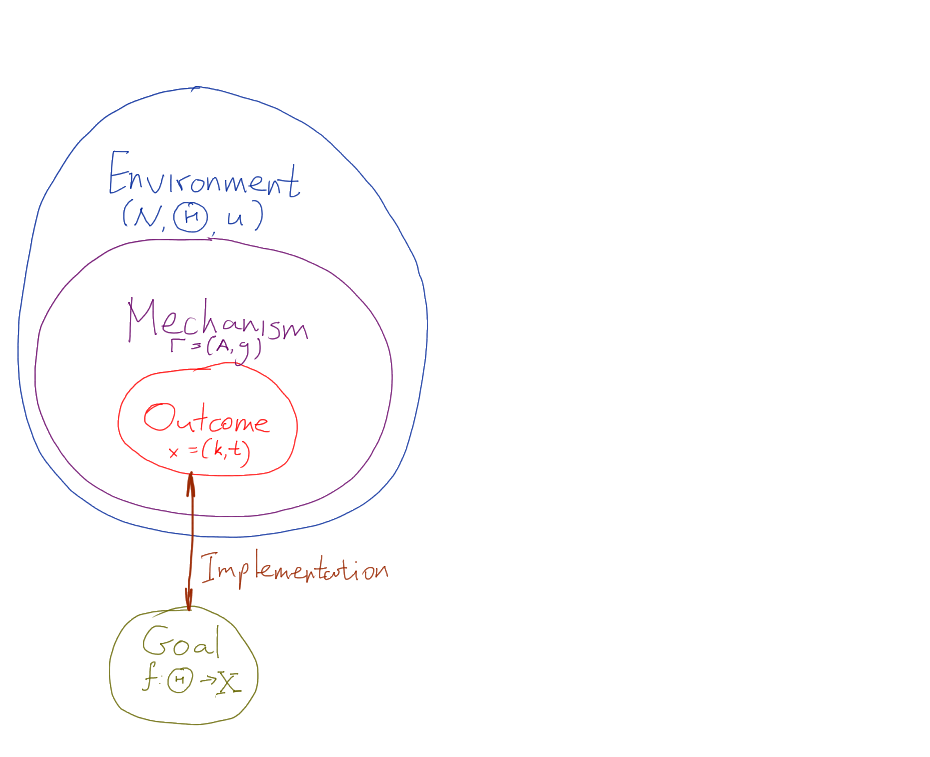
\includegraphics[scale=0.32]{pics/M7/MD_vs_ID_1}
\end{frame}


\begin{frame}
	\centering
	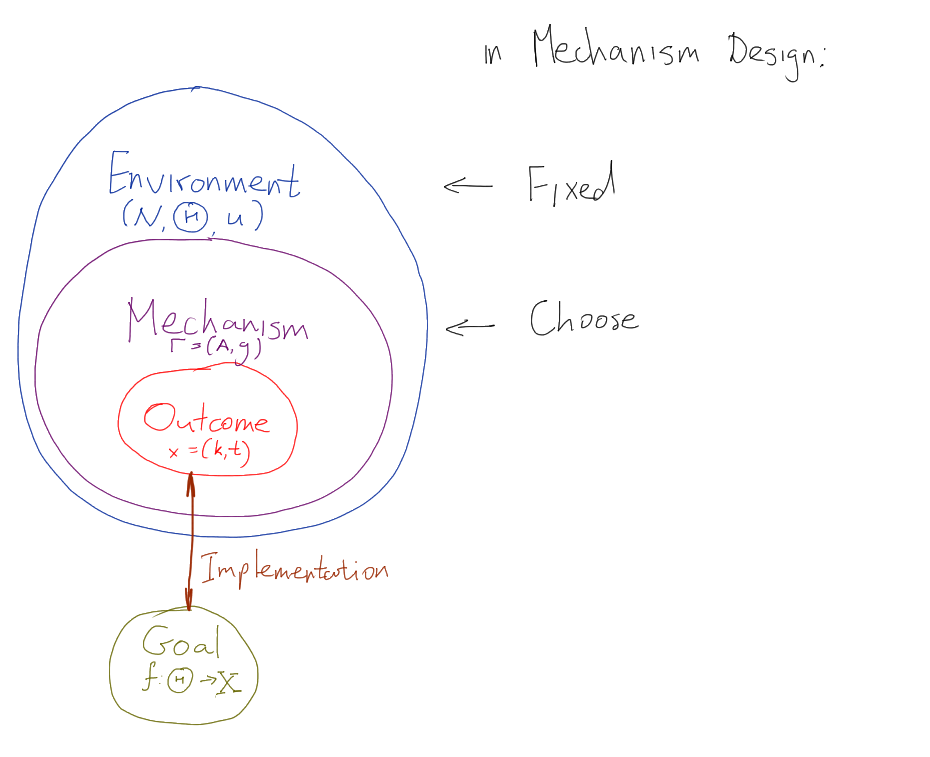
\includegraphics[scale=0.32]{pics/M7/MD_vs_ID_2}
\end{frame}


\begin{frame}
	\centering
	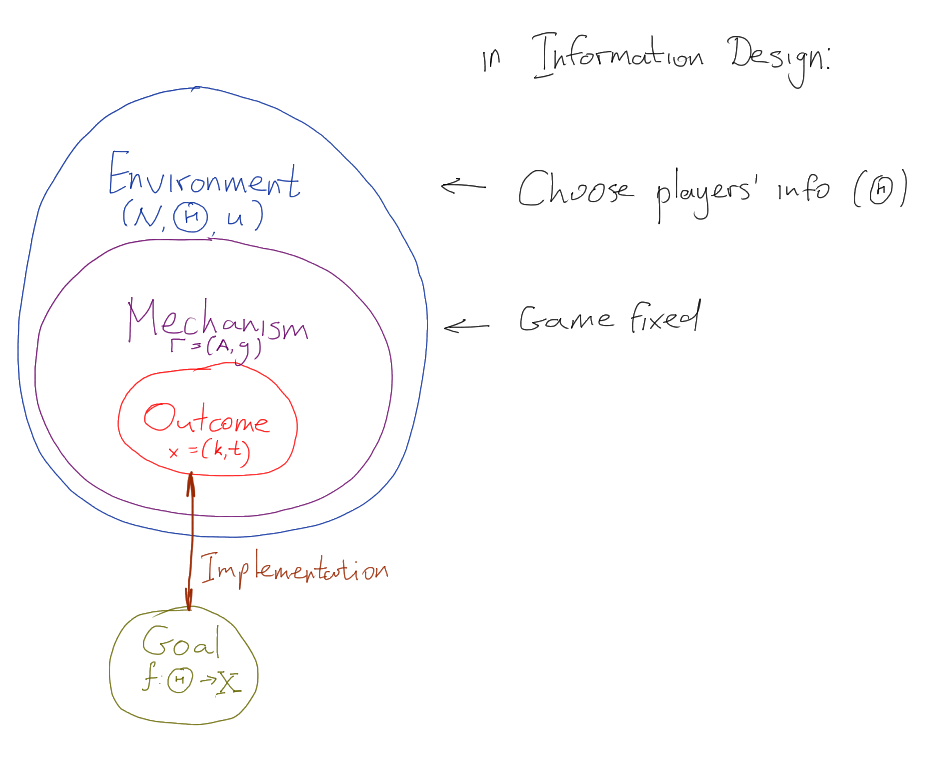
\includegraphics[scale=0.32]{pics/M7/MD_vs_ID_3}
\end{frame}


\begin{frame}{What is Information Design?}
\begin{itemize}
	\item In Mechanism design, we have:
	\begin{itemize}
		\item \alert{fixed} information and set of outcomes;
		\item \structure{choose} the game that agents play (available actions and their mapping to outcomes).
	\end{itemize}
	\item Information design (a.k.a. ``Bayesian Persuasion'') flips the problem completely:
	\begin{itemize}
		\item now have a \alert{fixed game} (actions and outcomes);
		\item can \structure{choose the information} that players have about their payoffs (and others' payoffs too!)
	\end{itemize}
	\item Alternatively, in the context of ``how to extract information from the player?'' problem:
	\begin{itemize}
		\item We've looked at settings when there's a fixed game between sender(s) and receiver (cheap talk, disclosure) and when receiver can design and commit to various incentive schemes.
		\item Now: effectively a communication game, where the \emph{sender} can credibly commit to a certain communication strategy.
	\end{itemize}
	\item This lecture very vaguely follows \cite{bergemann_information_2019}. \cite{kamenica_bayesian_2019} may also be useful.
\end{itemize}
\end{frame}


\begin{frame}{Setting}
\begin{itemize}
	\item There is some \structure{state} $\omega \in \Omega$, unknown to \emph{everyone} initially, common prior $\phi_0 \in \varDelta(\Omega)$.
	\item \alert{Players/receivers} $i \in \{1,...,N\}$ (we will mostly look at $N=1$);
	\begin{itemize}
		\item each player chooses an \structure{action} $a_i \in A_i$;
		\item player's \structure{utility} function is $v_i(a, \omega)$, where $a = (a_1, ..., a_N)$.
		\item To be clear: both $(A_1,...,A_N)$ and $(v_1,...,v_N)$ are \textbf{fixed} by the problem environment.
	\end{itemize}
	\item \alert{Designer/sender's} \structure{objective} function is $v_0(a, \omega)$.
	\item Designer chooses an \structure{experiment} $(\mu,M)$ where $\mu: \Omega \to \varDelta(M^N)$. 
	\\ (continued on the next slide)
\end{itemize}
\end{frame}
\note{
	Think ``state = type profile'' in terms of uncertainty, but now types are not known to players.
	
	Experiment is a distribution of signals that may or may not be informative about state... More in the following slides.
}


\begin{frame}{Experiments}
\begin{itemize}
	\item Designer chooses an \structure{experiment} $\mu: \Omega \to \varDelta(M^N)$.
	\item In words: an experiment produces, given state $\omega$, some distribution over messages $m_i$ for every player $i$.
	\begin{itemize}
		\item For a given $\omega$, $\mu(\omega)$ is a distribution over messages = a (mixed) messaging strategy. So the whole $\mu$ prescribes such a messaging strategy for every state $\omega$.
		\item Without commitment, $\mu(\omega)$ must be optimal for the sender given $\omega$. That would be a cheap talk model.
	\end{itemize}
	\item Player $i$ observes message $m_i$ generated by the experiment and uses it to update their belief $\phi$ about the state, which affects which action $a_i$ they will choose.
	\item The designer chooses an experiment to manipulate players' info $\rightarrow$ players' beliefs $\rightarrow$ players' actions.
\end{itemize}
\end{frame}


\begin{frame}{Experiments}
\begin{itemize}
	\item \textbf{Examples}:
	\begin{itemize}
		\item \emph{Perfectly revealing signals}: ($\Omega$ arbitrary and) $m_i = \omega$.
		\item \emph{Pooling signals}: ($\Omega \subseteq \mathbb{R}$ and) $m_i = 1$ if $\omega \geq 0$ and $m_i = 0$ if $\omega < 0$.
		\item \emph{Partially informative signals}: ($\Omega=\{L,R\}$ and) $m_i = C$ if $\omega = L$ and $m_i = 
		\begin{cases}
			C & \text{ w.p. }1/2; \\ R & \text{ w.p. }1/2
		\end{cases}$
		if $\omega=R$.
		\item \emph{Uninformative signals}: $m_i \sim F(M)$ where c.d.f. $F$ is \emph{independent} of $\omega$.
	\end{itemize}
	\item Distinction is made between \structure{private persuasion} where the designer can send a private signal to each player and \alert{public persuasion} where only public signals are available.
	\begin{itemize}
		\item Public signals are available under private persuasion, but not vice versa.
		\item Private persuasion is thus always weakly better for the designer.
	\end{itemize}
	\item Further, timing is important...
\end{itemize}
\end{frame}


\begin{frame}
	\centering
	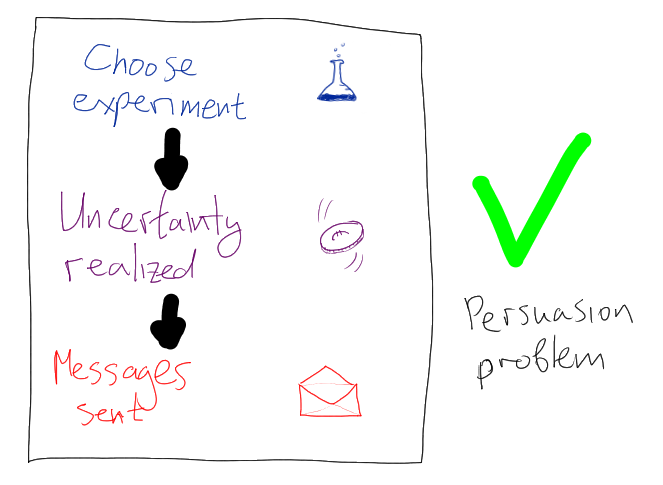
\includegraphics[scale=0.7]{pics/M7/timing1}
\end{frame}


\begin{frame}
	\centering
	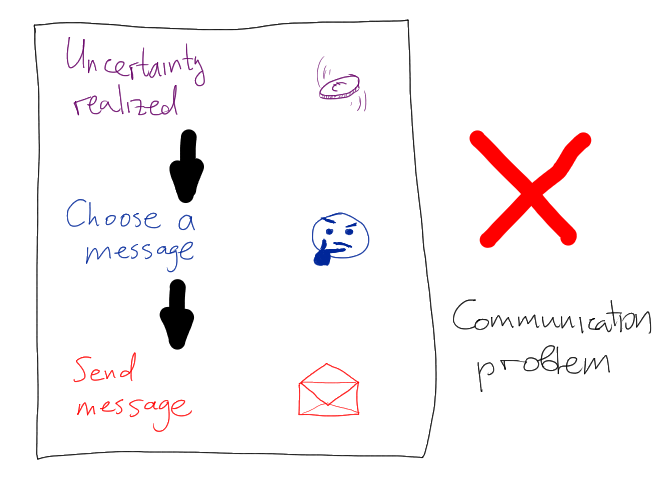
\includegraphics[scale=0.7]{pics/M7/timing2}
\end{frame}


\begin{frame}{Experiments}
\begin{itemize}
	\item It is crucial that the designer \alert{does not know $\omega$} when choosing $\mu$.
	\item Like in mechanism design, the designer publicly announces and \structure{commits} to $\mu$. 
	\\ I.e., can promise ex ante to reveal something not worth revealing ex post:
	%\item This commitment power allows the designer to commit ex ante to something that is not necessarily optimal ex post:
	\begin{itemize}
		\item e.g., commit to telling all truth and nothing but truth -- even if unfavorable facts may come up;
		\item or commit to giving no hints to players -- even if really want to reveal the state sometimes.
	\end{itemize}
	\item Without commitment -- if designer chooses a message \emph{after} learning $\omega$ -- we have a \alert{communication/cheap talk problem} (rather than information design problem).
	\begin{itemize}
		\item These are much more difficult to analyze, mostly due to linkages across states.
		\item E.g. a manager wants to boast high earnings to investors but does not want to reveal if earnings low. Without commitment, always reveals when earnings are high. Then if investors hear nothing, they infer that earnings are low -- communication in high-earning state imposes an informational externality on low-earning state.
	\end{itemize}
\end{itemize}
\end{frame}


\begin{frame}{What are ``experiments''?}
	Such a commitment to an experiment/communication strategy can be maintained via:
	\begin{itemize}
		\item \textbf{hardware/software}: the sender hardcodes the comm strategy into a device that observes the state and sends a corresponding message (example next slide)
		
		\item \textbf{blockchain smart contract}: special case of the software commitment above
		
		\item \textbf{reputation}: if sender \& receiver interact repeatedly, receiver can punish sender for deviating from an announced strategy if such deviations observable \citep{best_persuasion_2020}
	\end{itemize}
\end{frame}


\begin{frame}{Where  are ``experiments''? (1)}
	IRL \textbf{example} of such ``experiments'' (commitment to comm strategies) \citep{bondi_signal_2020}:
	\begin{itemize}
		\item \alert{Wildlife poaching} is a problem in many natural preserves. South Africa uses aerial drones with IR/video cameras to (1) detect poachers, (2) alert rangers in the vicinity, if any, and (3) alert poachers they've been detected, for deterrence.
		
		\item In this setting: $\omega \in \{ \text{detected, undetected} \} \times \{ \text{rangers coming, rangers not coming} \}$
		
		\item Messages (to poachers) are $m \in \{ \text{alert, no alert} \}$. Messaging strategy encoded in software = commitment.
		
		\item Conflict: want to let poachers know they are detected and rangers are coming in order to make them flee, but want the threat to be credible (i.e., not signal too often when no rangers are actually in range).
		
		\item The idea (tradeoff between deterrence and credibility) is common to ``\alert{security games}'': highway patrols, accounting audits, hacking detection, ...
	\end{itemize}
\end{frame}


\begin{frame}{Where  are ``experiments''? (2)}
	Other \textbf{examples} of such problems from \cite{kamenica_bayesian_2019} survey (refer to it for exact references):
	\begin{columns}
		\begin{column}{0.5\linewidth}
			\begin{itemize}
				\footnotesize
				\item financial sector stress tests (Goldstein \& Leitner 2018, Inostroza \&
				Pavan 2018, Orlov et al. 2018b), 
				
				\item grading in schools (Boleslavsky \& Cotton 2015, Ostrovsky \&
				Schwarz 2010), 
				
				\item employee feedback (Habibi 2018, Smolin 2017), 
				
				\item law enforcement deployment (Hernandez \& Neeman 2017, Lazear 2006, Rabinovich et al. 2015), 
				
				\item censorship (Gehlbach \& Sonin 2014), 
				
				\item entertainment (Ely et al. 2015), 
				
				\item financial over-the-counter markets (Duffie et al. 2017),
			\end{itemize}
		\end{column}
		\begin{column}{0.5\linewidth}
			\begin{itemize}
				\footnotesize
				\item voter coalition formation (Alonso \& Camara 2016b), 
				
				\item research procurement (Yoder 2018), 
				
				\item contests (Feng \& Lu 2016, Zhang \& Zhou 2016), 
				
				\item medical testing (Schweizer \& Szech 2019), 
				
				\item medical research (Kolotilin 2015), 
				
				\item matching platforms (Romanyuk \& Smolin 2019), 
				
				\item price discrimination (Bergemann et al. 2015), 
				
				\item financing (Szydlowski 2016), 
				
				\item insurance (Garcia \& Tsur 2018), 
				
				\item transparency in organizations (Jehiel 2015), 
				
				\item routing software (Das et al. 2017, Kremer et al. 2014).
			\end{itemize}
		\end{column}
	\end{columns}
	
\end{frame}


\begin{frame}{Two interpretations of Information Design}
\begin{itemize}
	\item There are two schools of thought in InfoDesign literature.
	\item The first takes the \structure{literal interpretation}, as presented above:
	\begin{itemize}
		\item there is some designer, who decides how to provide information.
		\item School led by Kamenica, most applications take this stand. %(even when commitment makes no sense).
	\end{itemize}
	\item The alternative is a \structure{metaphorical interpretation}:
	\begin{itemize}
		\item Suppose we are looking at some game or real-world interaction, but do not know what information is available to players.
		\item InfoDesign tools allow to describe the full set of possible outcomes for all possible information structures. 
		\item No explicit designer in this story.
		\item Note that in this story all players have common knowledge of the information structure in place, it is only us (the external observer) who do not know it. (Although there are sophisticated epistemologic arguments for why this is without loss.)
		\item Agenda pushed heavily by Morris.
	\end{itemize}
	\item The two also propose somewhat different approaches to solving the model, we will cover both.
\end{itemize}
\end{frame}



\section{Illustrative Example}

\begin{frame}{Illustrative example}
	\begin{columns}
		\begin{column}{0.5\linewidth}
			\begin{exampleblock}{The Witness}
				\begin{itemize}
					\item A suspect is on trial, accused of murder.
					%He is either guilty, or not: $\omega \in \{G,N\}$; let $\phi_0 = \mathbb{P} \{ \omega = G \}$ denote the common (judge's \& prosecutor's) prior belief (probability of being guilty).
					\item Judge must decide whether to convict or acquit him, wants to make the right decision.
					\item Prosecutor is paid per cases won, so wants to convict the suspect regardless of guilt.
					\item Prosecutor can call up a witness. What kind of witness should he summon?
				\end{itemize}
			\end{exampleblock}
		\end{column}
		\begin{column}{0.46\linewidth}
			
\includegraphics[scale=0.28]{pics/M7/miles}
		\end{column}
	\end{columns}
	\pause
	\centering
	Frame the above as an information design problem.
\end{frame}


\begin{frame}{Decyphering the example}
\begin{itemize}
	\item Designer = prosecutor.
	\item State $\omega \in \{G,N\}$ represents true guilt. 
	\item Let $\phi_0 = \mathbb{P} \{ \omega = G \}$ denote the common prior belief (probability that the prosecutor and the judge assign to the suspect being guilty).
	\item $N=1$ (judge), $A = \{g,n\}$ (verdicts ``guilty'', ``not guilty'');
	\pause
	\item The judge's utility is $v_1(a,\omega) = \mathbb{I} (a=\omega)$.
	\begin{itemize}
		\item You can model it in an asymmetric way too (convicting the innocent can be more or less costly than letting a criminal go).
	\end{itemize}
	\item The prosecutor's objective function is $v_0(a,\omega) = \mathbb{I} (a=G)$.
	\begin{itemize}
		\item Prefers the ``guilty'' verdict regardless of state.
	\end{itemize}
	\pause
	\item The witness was at a certain place on the night of murder -- this determines $\mu$
	\begin{itemize}
		\item If W was around the place of murder, can confirm or deny the suspect was there.
		\item if W was in a random pub, can do the same, but this conveys different information.
	\end{itemize}
\end{itemize}
\end{frame}


\begin{frame}{Example: timing}
	\begin{itemize}
		\item To be clear, the timing in this example (as well as in the general model) is as follows:
		\begin{enumerate}
			\item state $\omega$ is determined, observed by no one
			\item prosecutor chooses the witness $\mu$ and publicly commits to it
			\item witness reveals message $m$ to the court according to $\mu(m|\omega)$
			\item the judge observes $m$ and chooses decision $a$
			\item payoffs are realized
		\end{enumerate}
	\end{itemize}
\end{frame}


\begin{frame}{Example: 4: actions}
\begin{itemize}
	\item Start from the end (proceed by backwards induction):
	\item Let $\phi$ denote the judge's \structure{posterior belief} (after she observes $m$). What action does she choose?
	\item Denote $\hat{a}(\phi) \equiv \arg \max \mathbb{E}_{\phi(\omega)} [v_1(a,\omega)]$. If there are many optimal actions, choose the best for the prosecutor.
	\begin{itemize}
		\item For the first time ever we want to fix the tie-breaking rule. The reason will be evident later.
	\end{itemize}
	\pause
	\item In our example:
	\begin{equation*}
		\hat{a}(\phi) = \begin{cases}
			g & \text{ if } \phi \geq 1/2;
			\\
			n & \text{ if } \phi < 1/2.
		\end{cases}
	\end{equation*}
\end{itemize}
\end{frame}


\begin{frame}{Example: 3d: posteriors}
\begin{itemize}
	\item Knowing $\hat{a}(\phi)$ means we can write the prosecutor's utility as a function of $\phi$: let
	\vspace{-0.5em}
	\begin{equation*}
		V_0 (\phi) \equiv v_0(\hat{a}(\phi)) = \begin{cases}
			1 & \text{ if } \phi \geq 1/2;
			\\
			0 & \text{ if } \phi < 1/2.
		\end{cases}
	\end{equation*}
	\vspace{-1.5em}
	\pause
	\item By choosing an experiment $(\mu,M)$ the prosecutor induces some distribution $\tau$ over posteriors $\phi$. \textbf{Trick}: forget about $\mu$ and focus on this distribution $\tau$ as the choice object
	\begin{itemize}
		\item What if P could choose any distribution? Would want $\phi \geq 1/2$ always (after any message $m$).
		\item So if $\phi_0 \geq 1/2$ then optimal for P to do nothing (choose uninformative experiment).
		\item But the ideal is unattainable if $\phi_0 < 1/2$ because beliefs must be \alert{consistent}.
	\end{itemize}
	\pause
	\item \structure{Belief consistency}: $\mathbb{E}_\mu \phi = \phi_0$ (Law of iterated expectations). \\
	Expectation is taken from the ex ante perspective.
	\begin{itemize}
		\item \alert{Remark}: always keep track of perspective. In ID you have ex ante expectations, expectations conditional on $m$, expectations conditional on $\omega$ -- easy to get lost!
	\end{itemize}
\end{itemize}
\end{frame}


\begin{frame}{Example: 3c: feasible distributions}
\begin{itemize}
	\item Let us try to find the \structure{best (for P) distribution} of posteriors $\phi$ such that $\mathbb{E} \phi = \phi_0 < 1/2$.
	\begin{itemize}
		\item It only matters for $V_0(\phi)$ whether $\phi < 1/2$ or $\phi \geq 1/2$.
		\item So suppose there are two possible posteriors induced by the experiment: $\phi_1 < 1/2$ and $\phi_2 \geq 1/2$, occurring with respective probabilities $\tau_1$ and $\tau_2 = 1 - \tau_1$. 
		\item Consistency pins the probabilities exactly:
		\begin{align} \nonumber
			\tau_1 \phi_1 + (1-\tau_1) \phi_2 = \phi_0
			\\ \label{eq:ID_cons}
			\Leftrightarrow \structure{\tau_1 = \frac{\phi_2 - \phi_0}{\phi_2 - \phi_1}} = 1 - \frac{\phi_0 - \phi_1}{\phi_2 - \phi_1}
		\end{align}
		(Note that this also implies that $\phi_1 < \phi_0$, since must have $\tau_1 \in [0,1]$.)
		\item (This is not the optimal distribution yet, we only computed $\tau$ \emph{given} $\phi_1,\phi_2$ -- but we also want to find the optimal values of $\phi_1,\phi_2$)
	\end{itemize}
\end{itemize}
\end{frame}


\begin{frame}{Example: 3b: optimal distribution}
	\begin{itemize}
		\item P gets payoff $1$ whenever $\phi_2$ is induced and $0$ in case of $\phi_1$:
		\vspace{-0.5em}\begin{align*}
			\mathbb{E}_\phi V_0 (\phi) = \tau_1 \cdot 0 + (1-\tau_1) \cdot 1 = 1-\tau_1
		\end{align*}\vspace{-1.5em}
		\begin{itemize}
			\item Hence want to choose $(\phi_1,\phi_2)$ so as to minimize $\tau_1$ subject to \eqref{eq:ID_cons}, $\phi_1 \in [0, \phi_0)$, and $\phi_2 \in [1/2, 1]$.
			\item The solution is \structure{$\phi_1 = 0$, $\phi_2 = 1/2$}. (The objective function is increasing in both $\phi_1$ and $\phi_2$, so FOCs never hold -- thus you only need to check the edges of the domain.)
		\end{itemize}
	
		\item So \alert{the optimal distribution is}: induce posterior $\phi_1 = 0$ with probability $\tau_1 = 1-2\phi_0$ and posterior $\phi_2 = 1/2$ with probability $\tau_2 = 2 \phi_0$.
		\begin{itemize}
			\item This yields utility $2 \phi_0$ to the designer.
		\end{itemize}
	\end{itemize}
\end{frame}


\begin{frame}{Example: 3a: from distribution to experiment}
\begin{itemize}
	\item Final part: how to design \alert{an experiment} $(\mu,M)$ to induce the desired distribution $\tau$? 
	\begin{itemize}
		\item (It can be shown that this problem always has a solution if $\tau$ is \emph{consistent} with the prior $\phi_0$.)
		\item Have two posteriors so use two messages: $M = \{g,n\}$, where $n$ will induce posterior $\phi_1$, and $g$ corresponds to $\phi_2$.
		\item Let $p(m|\omega)$ denote the probability that message $m$ is sent in state $\omega$. We then need to solve the following system w.r.t. $p(m|\omega)$:
		\begin{align*}
			\frac{\phi_0 p(n|G)}{\phi_0 p(n|G) + (1-\phi_0) p(n|N)} &= \phi_1 = 0
			\\
			\frac{\phi_0 p(g|G)}{\phi_0 p(g|G) + (1-\phi_0) p(g|N)} &= \phi_2 = 1/2
			\\
			p(n|N) + p(g|N) &= 1
			\\
			p(n|G) + p(g|G) &= 1
		\end{align*}
		First two equalities ensure that messages $b$ and $g$ induce exactly the right posteriors (and follow from Bayes' rule); the last two are feasibility constraints (one of the two messages must always be sent).
	\end{itemize}
\end{itemize}
\end{frame}


\begin{frame}{Example: optimal experiment}
\begin{itemize}
	\item \textbf{The solution} is given by:
	\vspace{-1em}\begin{align*}
		p(g|N) &= \frac{\phi_0}{1-\phi_0} = 1-p(n|N)
		\\
		p(g|G) &= 1 = 1-p(n|G)
	\end{align*}\vspace{-2em}
	\begin{itemize}
		\item i.e., in state $\omega=G$ always send $m=g$;
		\item in state $\omega=N$ mix between sending $m=g$ w.p. $\frac{\phi_0}{1-\phi_0}$ and $m=n$ w.p. $\frac{1-2\phi_0}{1-\phi_0}$,
	\end{itemize}
	\item In other words, the optimal strategy is:
	\begin{itemize}
		\item if \structure{state favorable} to prosecutor then disclose it \structure{truthfully};
		\item if \alert{state bad} for prosecutor then try to \alert{obfuscate} it.
		\item Need \alert{commitment} to mix in $\omega=N$: message $m=g$ gives higher payoff, so without commitment the prosecutor would never send $m=n$.
	\end{itemize}
	\item The judge is granted full confidence when taking action that is undesirable for designer; is made barely indifferent when taking action desired by the designer.
\end{itemize}
\end{frame}



\section{General Approach A: Concavification}

\begin{frame}{Setting (reminder)}
\begin{itemize}
	\item There is some \structure{state} $\omega \in \Omega$, unknown to everyone initially, common prior $\phi_0 \in \varDelta(\Omega)$.
	\item \alert{Players} $i \in \{1,...,N\}$ (we will mostly look at $N=1$);
	\begin{itemize}
		\item each player chooses an \structure{action} $a_i \in A_i$;
		\item player's \structure{utility} function is $v_i(a, \omega)$, where $a = (a_1, ..., a_N)$.
	\end{itemize}
	\item \alert{Designer's} \structure{objective} function is $v_0(a, \omega)$.
	\item Designer chooses an \structure{experiment} $(\mu,M)$ where $\mu: \Omega \to \varDelta(M^N)$.
\end{itemize}
\end{frame}


\begin{frame}{Timing}
	\begin{enumerate}
		\item \structure{Experiment} $(\mu,M)$ is selected by the designer.
		\item \structure{Message} $m$ is generated by the experiment according to $\mu(m|\omega)$ (where $\omega$ is the true realized state). Every player $i$ updates \structure{beliefs}.
		\begin{itemize}
			\item Given message $m_i$, the probability that \structure{$i$'s posterior belief} assigns to any $\omega$ is given by:
			\begin{align*}
				\phi_i(\omega|m_i) = \frac{\mu(m_i|\omega)\phi_0(\omega)}{\sum_{\omega' \in \Omega} \mu(m_i|\omega')\phi_0(\omega')}
			\end{align*}
			
			\pause
			\item Note that \alert{Belief consistency} is then a direct consequence of the law of total probability.
			\\
			Pick some $\omega$ and calculate the expected (over $m_i$) probability that $\phi_i$ will assign to it:
			\begin{align*}
				\alert{\mathbb{E}_\mu [\phi_i(\omega|m_i)|\phi_0] }
				%&= \sum_{m_i \in M_i} \sum_{\omega' \in \Omega} \phi_i(\omega|m_i) \mu(m_i|\omega') \phi_0(\omega') 
				%\\
					&= \sum_{m_i \in M_i} \phi_i(\omega|m_i) \cdot \left[ \sum_{\omega' \in \Omega} \mu(m_i|\omega') \phi_0(\omega') \right] 
				\\
				\visible<3->{
					&= \sum_{m_i \in M_i} \frac{\mu(m_i|\omega)\phi_0(\omega)}{\structure<4>{\sum_{\omega' \in \Omega} \mu(m_i|\omega')\phi_0(\omega')}} \cdot \structure<4>{ \left[ \sum_{\omega' \in \Omega} \mu(m_i|\omega') \phi_0(\omega') \right] }
				}
				\\
				\visible<5->{
					&= \sum_{m_i \in M_i} \mu(m_i|\omega)\phi_0(\omega) \alert{= \phi_0(\omega)}
				}
			\end{align*}
		\end{itemize}
	\end{enumerate}
\end{frame}


\begin{frame}{Timing}
	\begin{enumerate}
		\item \structure{Experiment} $(\mu,M)$ is selected by the designer.
		\item \structure{Message} $m$ is generated by the experiment according to $\mu(m|\omega)$ (where $\omega$ is the true realized state). Every player $i$ updates \structure{beliefs}.
		\begin{itemize}
			\item Given message $m_i$, the probability that \structure{$i$'s posterior belief} assigns to any $\omega$ is given by:
			\begin{align*}
				\phi_i(\omega|m_i) = \frac{\mu(m_i|\omega)\phi_0(\omega)}{\sum_{\omega' \in \Omega} \mu(m_i|\omega')\phi_0(\omega')}
			\end{align*}
			
			\item In general, every $i$ also needs to form beliefs over others' messages(=``types''), since $m_j$ determine $\phi_j$ and $a_j$.
			\begin{itemize}
				\item Step only relevant if: (1) $N>1$ and (2) private persuasion is available to designer.
				\item We will not look carefully at this step.
			\end{itemize}
		\end{itemize}
		\item Every $i$ selects optimal/equilibrium \structure{action} $\hat{a}_i$ given their beliefs.
	\end{enumerate}
\end{frame}

\begin{frame}{Actions are irrelevant}
\begin{itemize}
	\item Restrict attention to \alert{public experiments}
	\begin{itemize}
		\item so all players always receive same message $m$ and end up with \structure{same posterior} belief $\phi \in \varDelta (\Omega)$.
		\item I do not think this general approach can easily account for private experiments.
	\end{itemize}
	\item Let $\hat{a}(\phi)$ denote an equilibrium (BNE) strategy profile in a game where all $i$ share belief $\phi$.
	\begin{itemize}
		\item Same as in the example, except now want equilibrium rather than just maximizer.
		\item If many equilibria, select designer-best.
	\end{itemize}
	\item Define $V_0 (\phi) \equiv \mathbb{E}_{\phi} \left[v_0 (\hat{a}(\phi), \omega)\right]$.
	\begin{itemize}
		\item Again, posterior $\phi$ completely defines the designer's objective function.
		\item Expectation needed because $v_0$ depends on $\omega$ in general.
		\item Expectation is w.r.t posterior $\phi$. Why not prior $\phi_0$?
	\end{itemize}
\end{itemize}
\end{frame}


%\begin{frame}{Posteriors}
%\begin{itemize}
%	\item Let $\phi_k = \phi (\omega | m_k)$ denote the players' shared posterior belief over states upon observing public message $m_k$:
%	\begin{align*}
%		\phi_k (\omega) = \frac{\phi_0(\omega) \mu(m_k|\omega)}{\sum_{\omega' \in \Omega} \phi_0 (\omega') \mu(m_k | \omega')}
%	\end{align*}
%	\item Let $\tau \in \varDelta(\varDelta(\Omega))$ denote the \structure{distribution over posteriors} $\phi_k$ induced by experiment $\mu$ (from the ex ante perspective).
%	\item Belief consistency / LIE: $\mathbb{E}_\tau \phi_k = \phi_0$
%	\begin{itemize}
%		\item from the ex ante perspective.
%	\end{itemize}
%\end{itemize}
%\end{frame}


\begin{frame}{Distributions over posteriors}
	\begin{itemize}
		\item As we saw, any experiment $(\mu,M)$ induces a \structure{distribution over posteriors} $\phi$. Denote it as $\tau \in \varDelta(\varDelta(\Omega))$.
		\begin{itemize}
			\item Under public persuasion, $\tau$ is the same for all players.
			\item In particular, the [unconditional] probability of posterior $\phi$ occurring under $\mu$ is:
			\begin{align*}
				\tau(\phi) = \begin{cases}
					\sum_{\omega' \in \Omega} \mu(m|\omega') \phi_0(\omega') & \text{ where $m$ is s.t. } \phi(\omega|m)=\phi;
					\\
					0 & \text{ if no such $m$ exists}.
				\end{cases}
			\end{align*}
		\end{itemize}
	
		\item Remember belief consistency: $\mathbb{E}_\mu \phi = \sum_{m \in M} \phi \tau(\phi) = \phi_0$.
	\end{itemize}
\end{frame}


\begin{frame}{Direct Experiments}
\begin{itemize}
	\item Note that messages' \structure{only} purpose is to induce some posterior. So we can w.l.o.g. focus on experiments which directly tell the player what posterior she must have upon hearing this message:
	\begin{definition}[Direct Experiment A]
		A \structure{direct} experiment is $(\mu,M)$ such that $M = \varDelta(\Omega)$.
	\end{definition}
	\item For the player to actually arrive at beliefs prescribed by a direct experiment, the experiment must be consistent:
\end{itemize}
\begin{definition}
	A direct experiment $(\mu,\varDelta(\Omega))$ is \alert{consistent} if $\mathbb{E}_\tau m_k = \phi_0$.
\end{definition}
\end{frame}


\begin{frame}{Revelation Principle}
\begin{theorem}[Revelation Principle A]
	\begin{itemize}
		\item For \structure{any experiment} $(\mu,M)$ there exists an equivalent \alert{credible consistent} experiment $(\mu,\varDelta(\Omega))$.
		
		\item For any consistent \structure{distribution} $\tau \in \varDelta(\varDelta(\Omega))$ there exists \alert{an experiment} $(\mu,M)$ that induces it.
	\end{itemize}
\end{theorem}
\begin{itemize}
	\item So instead of maximizing $V_0$ over all possible experiments $(\mu,M)$ we can maximize over the set of consistent distributions $\tau$, which is a slightly easier problem.
	\item This is what we did in the example, but now we know this is a way we can always go.
	\item From this point onwards, I will also call any consistent distribution $\tau$ an experiment.
\end{itemize}
\end{frame}


\begin{frame}{Concavification}
\begin{itemize}
	\item So how do we find the optimal experiment $\tau^{opt} \in \arg \max_{\tau} \left\{\mathbb{E}_\tau V_0(\phi) \right\}$?
	\pause
	\item Using the following scary object:
	\begin{definition}[Concave closure]
		Function $V_0^*(\phi)$ is a \alert{concave closure} of function $V_0(\phi)$ if it is the pointwise smallest concave function among those that satisfy $V_0^*(\phi) \geq V_0(\phi)$ for all $\phi$.
	\end{definition}
	\item Equivalent definition:
	\begin{align*}
		V_0^*(\phi) \equiv \sup \{ z | (\phi,z) \in co(V_0) \}
	\end{align*}
	where $co(V_0)$ is the convex hull of the graph of $V_0$. $V^*_0$ is then an upper envelope of this convex hull.
	%\item Recall that $V_0(\phi)$ is the designer's payoff from inducing posterior $\phi$. Call its concavification $V_0^*(\phi)$ the \structure{value function} of the designer. Why? See next slide.
	\item Equivalent definition: $V_0^*$ is the shape that the blanket takes when you throw it over $V_0$.
\end{itemize}
\end{frame}


%\begin{frame}{Concavification: example}
%\begin{center}
%	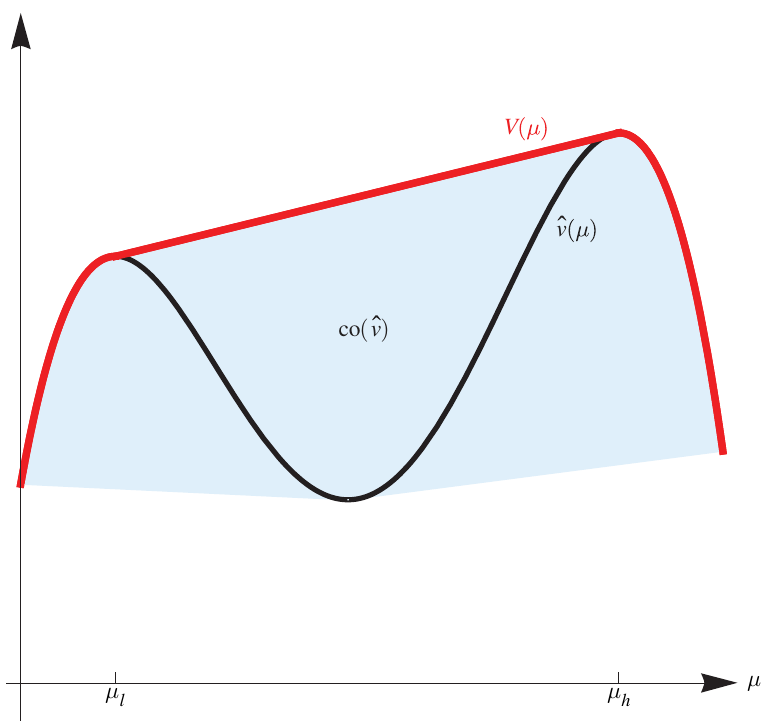
\includegraphics[scale=0.25]{pics/ID_concav.png}
%	
%	(Notation is different but you get the idea.)
%\end{center}
%\end{frame}


\begin{frame}
	\centering
	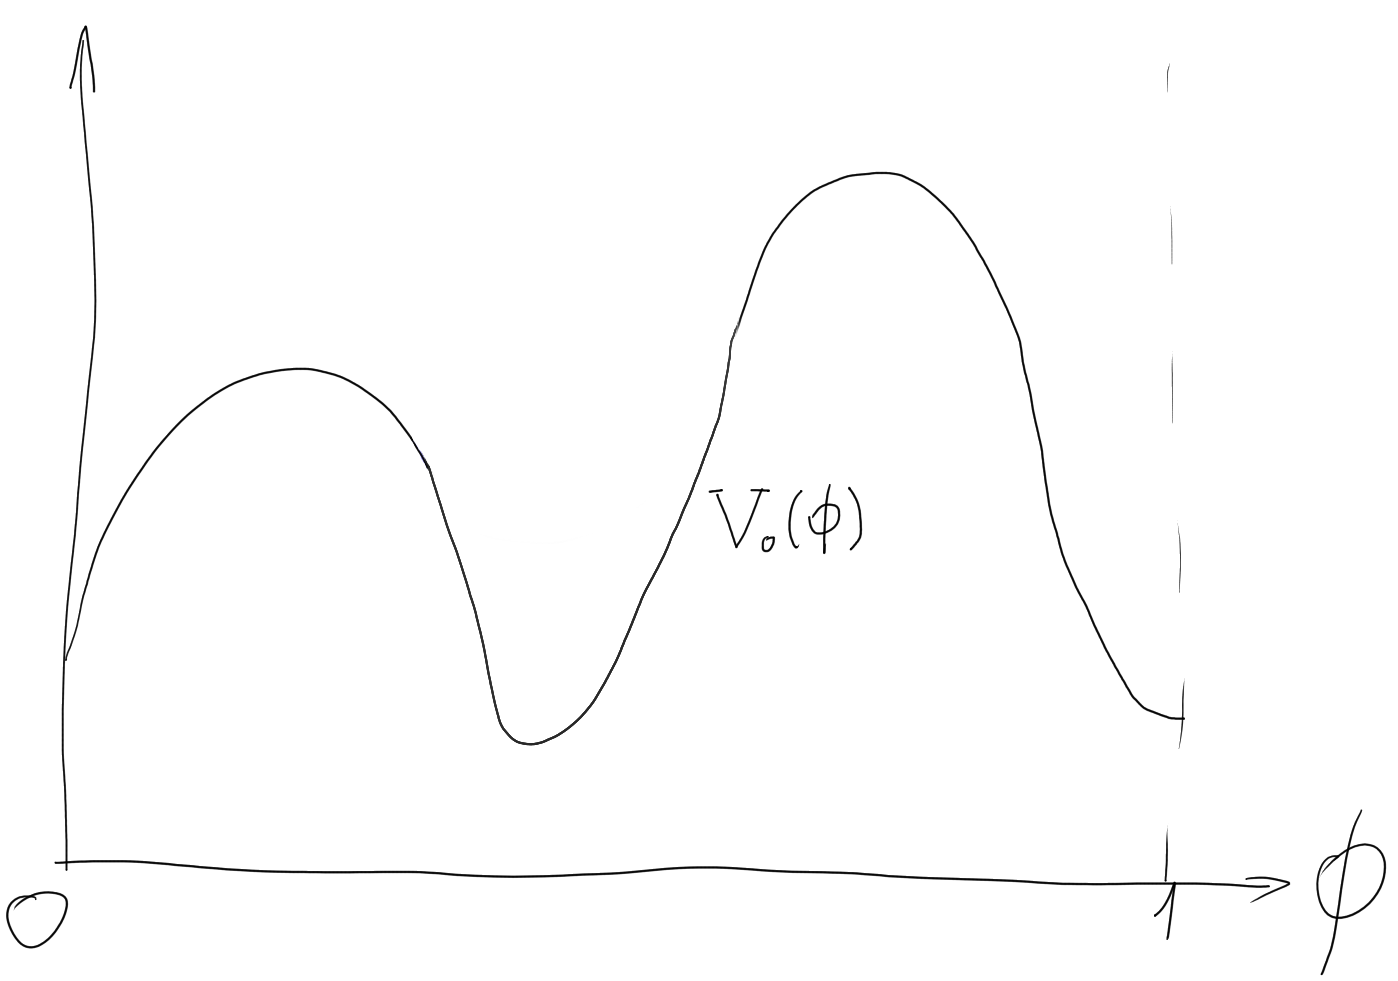
\includegraphics[scale=0.3]{pics/M7/concav1.png}
\end{frame}


\begin{frame}
	\centering
	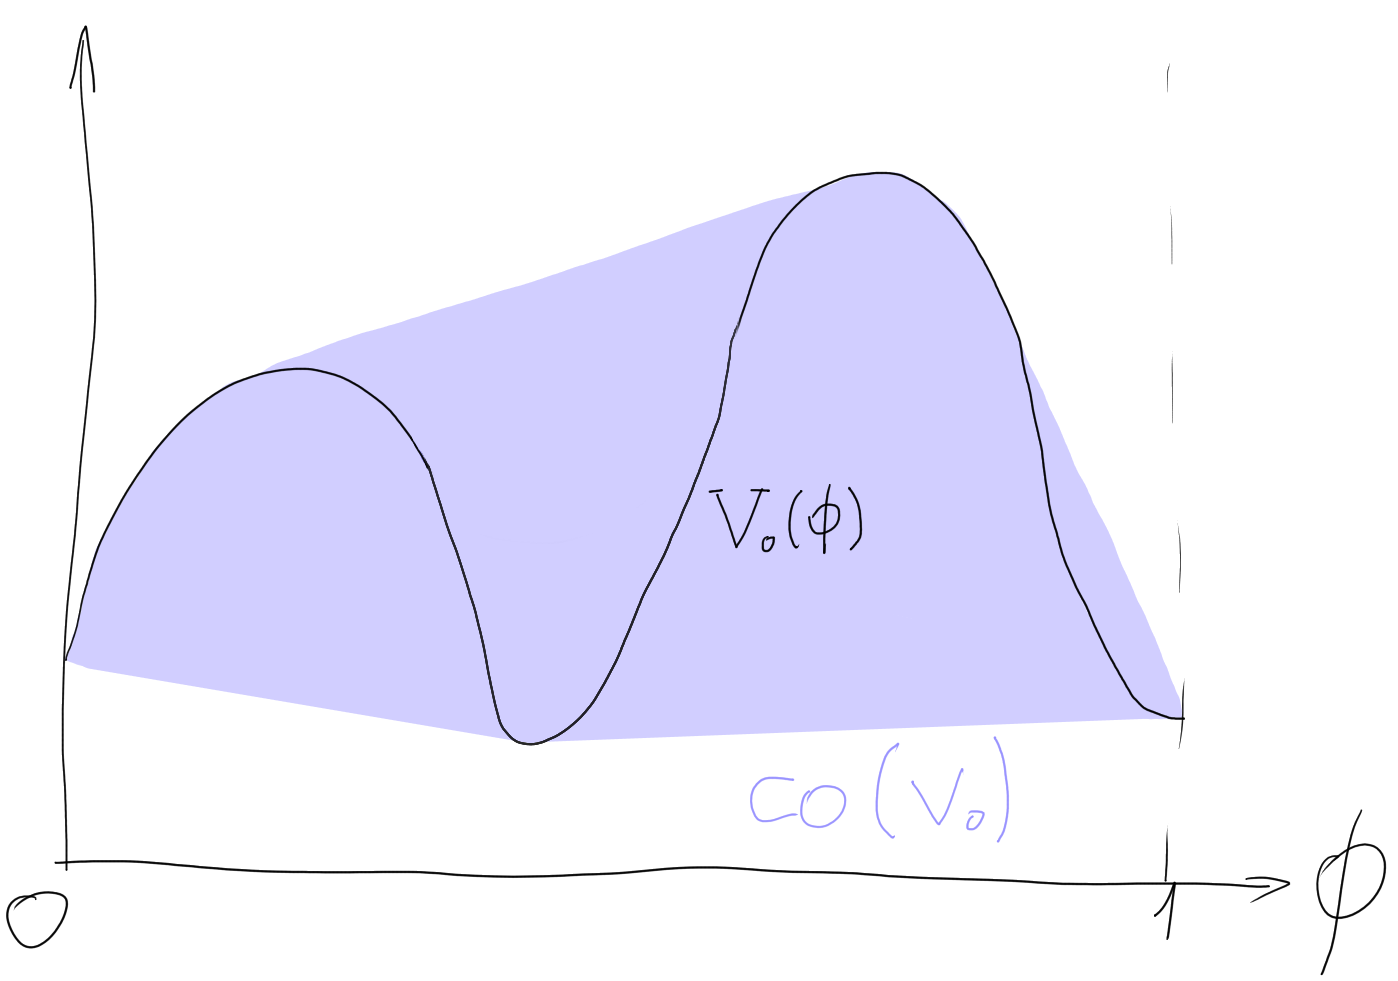
\includegraphics[scale=0.3]{pics/M7/concav2.png}
\end{frame}


\begin{frame}
	\centering
	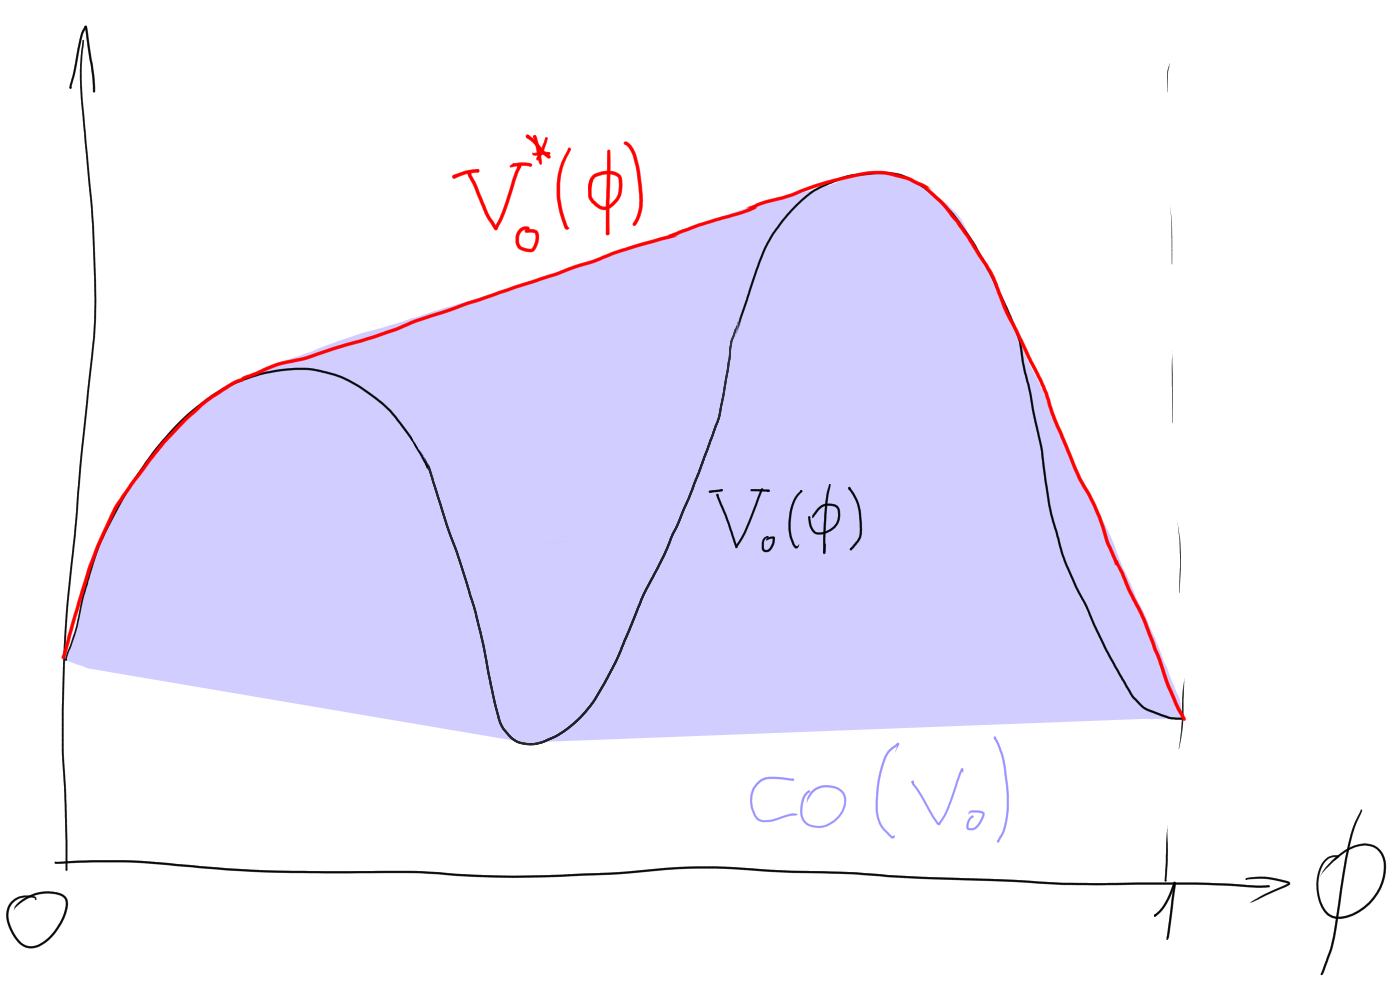
\includegraphics[scale=0.3]{pics/M7/concav3.png}
\end{frame}


\begin{frame}{Optimal experiment: payoff}
\begin{theorem}[Kamenica \& Gentzkow]
	The payoff the designer obtains from the optimal experiment is given by $V_0^*(\phi_0)$, where $V_0^*$ is the concave closure of $V_0$.
\end{theorem}
\begin{itemize}
	\item If $V_0^*(\phi_0) = V_0(\phi_0)$ then trivial (uninformative) experiment is optimal given prior $\phi_0$.
\end{itemize}
\end{frame}


\begin{frame}{Optimal experiment: cookbook}
\begin{itemize}
	\item If $V_0^*(\phi_0) > V_0(\phi_0)$ then you need to find a set of points \structure{$\{\phi_1, ..., \phi_K\}$} such that:
	\begin{itemize}
		\item $\phi_0 \in co\left(\{\phi_1, ..., \phi_k\}\right)$, meaning $\phi_0 = \sum_k \tau_k \phi_k$ for some weights $\tau_k$ ($\tau_k \geq 0$, $\sum_k \tau_k = 1$);
		\item $V_0^*(\phi_k) = V_0(\phi_k)$;
		\item $V_0^*(\phi_0) = \sum_k \tau_k V_0^*(\phi_k)$.
	\end{itemize}
	\item These $\phi_k$ will be the \structure{posteriors(=messages)} in the optimal experiment $\tau$.
	\item You can then use all $(\tau_k,\phi_k)$ to derive the \structure{conditional probabilities $\mu(m_k | \omega)$} of sending each message $m_k$ in each state $\omega$;
	\begin{itemize}
		\item use Bayes' rule + feasibility, as we did in the example.
	\end{itemize}
	\item Congratulations, you have just information designed.
\end{itemize}
\end{frame}


\begin{frame}{Back to example}
\begin{columns}
	\begin{column}{0.5\textwidth}
		\begin{center}
			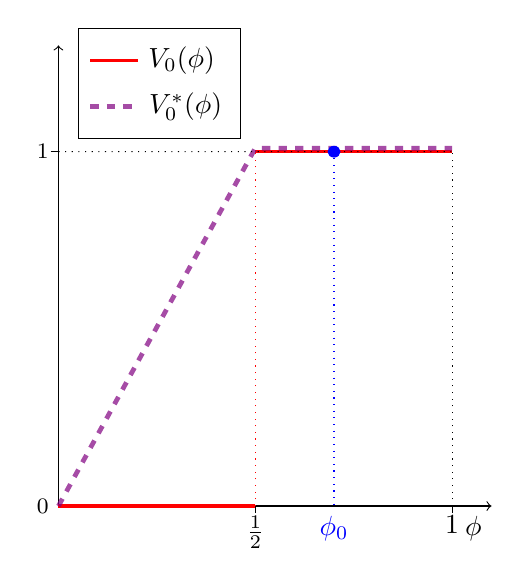
\begin{tikzpicture}[xscale=5,yscale=4.5,
				piline/.style={line width=0.4mm, red}
				]
				\draw[->] (0,0) -- (1.1,0) node[below left]{$\phi$};
				\draw[->] (0,0) -- (0,1.3);% node[below left]{$V_0^*(\phi)$};
				\draw (0,0) node[left]{\footnotesize $0$};
				
				% Plot
				% Pi
				\draw[piline] (0,0) -- (0.5,0);
				\draw[red,dotted] (0.5,0) -- (0.5,1);
				\draw[piline] (0.5,1) -- (1,1);
				
				\draw[line width=0.6mm, violet, opacity=0.7, dashed] (0,0) -- (0.5,1.01) -- (1,1.01);
				
				% Ticks
				% x axis
				\draw (0.5,0) coordinate(q1) node[below ]{$\frac{1}{2}$};
				\draw (q1) ++(0,-0.02) -- ++(0,0.02);
				
				\draw (1,0) coordinate(q3) node[below]{$1$};
				\draw (q3) ++(0,-0.02) -- ++(0,0.02);
				\draw[dotted] (1,0) -- (1,1);
				
				% y axis
				\draw (0,1) coordinate(u2) node[left]{\footnotesize $1$};
				\draw (u2) ++(-0.02,0) -- ++(0.02,0);
				\draw[dotted] (u2) -- (1,1);
				
				%Legend
				\matrix [draw, fill=white, below right] at (0.05,1.35) {
					\draw [piline] ++(-0.3,0) -- ++(0.6,0) node[black,right] {$V_0(\phi)$}; \\
					\draw [line width=0.6mm, violet, opacity=0.7, dashed] ++(-0.3,0) -- ++(0.6,0) node[black,right,opacity=1] {$V_0^*(\phi)$}; \\
				};
				
				\filldraw[blue] (0.7,1) circle(0.015);
				\draw[blue,dotted] (0.7,1) -- (0.7,0) node[below]{$\phi_0$};
			\end{tikzpicture}
		\end{center}
	\end{column}
	\begin{column}{0.5\textwidth}
		{\small
			\begin{itemize}
				\item If $\phi_0 \geq 1/2$ then $V_0^*(\phi_0) = V_0(\phi_0)$,
				\item so trivial mechanism is optimal.
			\end{itemize}
		}
	\end{column}
\end{columns}
\end{frame}


\begin{frame}{Back to example}
\begin{columns}
	\begin{column}{0.5\textwidth}
		\begin{center}
			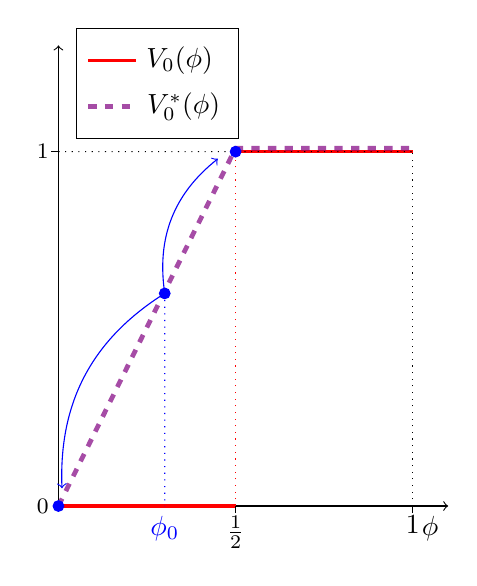
\begin{tikzpicture}[xscale=4.5,yscale=4.5,
				piline/.style={line width=0.4mm, red}
				]
				\draw[->] (0,0) -- (1.1,0) node[below left]{$\phi$};
				\draw[->] (0,0) -- (0,1.3);% node[below left]{$V_0^*(\phi)$};
				\draw (0,0) node[left]{\footnotesize $0$};
				
				% Plot
				% Pi
				\draw[piline] (0,0) -- (0.5,0);
				\draw[red,dotted] (0.5,0) -- (0.5,1);
				\draw[piline] (0.5,1) -- (1,1);
				
				\draw[line width=0.6mm, violet, opacity=0.7, dashed] (0,0) -- (0.5,1.01) -- (1,1.01);
				
				% Ticks
				% x axis
				\draw (0.5,0) coordinate(q1) node[below]{$\frac{1}{2}$};
				\draw (q1) ++(0,-0.02) -- ++(0,0.02);
				
				\draw (1,0) coordinate(q3) node[below]{$1$};
				\draw (q3) ++(0,-0.02) -- ++(0,0.02);
				\draw[dotted] (1,0) -- (1,1);
				
				% y axis
				\draw (0,1) coordinate(u2) node[left]{\footnotesize $1$};
				\draw (u2) ++(-0.02,0) -- ++(0.02,0);
				\draw[dotted] (u2) -- (1,1);
				
				%Legend
				\matrix [draw, fill=white, below right] at (0.05,1.35) {
					\draw [piline] ++(-0.3,0) -- ++(0.6,0) node[black,right] {$V_0(\phi)$}; \\
					\draw [line width=0.6mm, violet, opacity=0.7, dashed] ++(-0.3,0) -- ++(0.6,0) node[black,right,opacity=1] {$V_0^*(\phi)$}; \\
				};
				
				\filldraw[blue] (0.3,0.6) coordinate(p0) circle(0.015);
				\draw[blue,dotted] (p0) -- (0.3,0) node[below]{$\phi_0$};
				\draw[->,blue] (p0) to[bend left] (0.45,0.98);
				\filldraw[blue] (0.5,1) circle(0.015);
				\draw[->,blue] (p0) to[bend right] (0.01,0.05);
				\filldraw[blue] (0,0) circle(0.015);
			\end{tikzpicture}
		\end{center}
	\end{column}
	\begin{column}{0.5\textwidth}
		{\small
			\begin{itemize}
				\item If $\phi_0 < 1/2$ then $V_0^*(\phi_0) > V_0(\phi_0)$.
				\item Decompose $\phi_0$ into points such that $V_0^*(\phi) = V_0(\phi)$, namely $\phi_1 = 0$ and $\phi_2 = 1/2$
				\item which is exactly what we did when solving the example.
			\end{itemize}
		}
	\end{column}
\end{columns}
\end{frame}


\section{General Approach B: Correlated Equilibria}

\begin{frame}{Introduction}
\begin{itemize}
	\item Kamenica's ``concavification'' approach yields a nice visual representation of what ``Bayesian persuasion'' entails.
	\item But it is not very convenient to use in applications.
	\begin{itemize}
		\item Concavification is a very graphical concept.
		\item Easy to draw a picture for one-dimensional belief $\phi$ (two states),
		\item in principle you can draw one in three dimensions (three states),
		\item but with more states things become problematic.
	\end{itemize}
	\item But there is another, more boring but also more effective approach that links Information Design to an old literature on Correlated Equilibria.
	\begin{itemize}
		\item You can read more about it in Bergemann \& Morris (2019) survey.
	\end{itemize}
\end{itemize}
\end{frame}


\begin{frame}{Revelation Principle B}
\begin{itemize}
	\item In the previous approach, message $m$ prescribed the \structure{posterior belief} that a player must update to upon receiving that message.
	\item Now let it prescribe an \alert{action} that a player must take: 
	
	A \alert{decision rule} is $\sigma: \Omega \to \varDelta(A)$.
	\begin{itemize}
		\item Given state $\omega$, give an action recommendation to every player.
		\item Recommendations may be random given state, and be \structure{correlated} across players.
	\end{itemize}
	\item We will use decision rules as yet another representation of an experiment, along with $(\mu,M)$ -- message distribution, and $\tau$ -- distribution of posteriors.
	\begin{itemize}
		\item Every experiment induces some decision rule. Need to understand which decision rules can be implemented using some experiment.
	\end{itemize}
	\item Remark: we are no longer constrained to public experiments, now assume that messages are \structure{private}.
\end{itemize}
\end{frame}


\begin{frame}{Obedience}
\begin{definition}
	Decision rule $\sigma$ satisfies \alert{obedience} if for all $i$ and $a_i,a'_i \in A_i$:
	\begin{align*}
		\sum_{a_{-i},\omega} v_i ((a_i,a_{-i}), \omega) \sigma ((a_i,a_{-i}) | \omega) \phi_0(\omega) \geq
		\\
		\geq \sum_{a_{-i},\omega} v_i ((a'_i,a_{-i}), \omega) \sigma ((a_i,a_{-i}) | \omega) \phi_0(\omega) 
	\end{align*} 
\end{definition}
\begin{itemize}
	\item In words, when $i$ receives a recommendation to play $a_i$, following it must be better than playing any other $a'_i$ -- like our usual IC conditions
\end{itemize}
\end{frame}


\begin{frame}{Optimal experiment}
\begin{theorem}[Bergemann \& Morris]
	A decision rule $\sigma$ can be induced by an experiment if and only if $\sigma$ satisfies obedience.
\end{theorem}
\begin{itemize}
	\item The designer's problem then is choosing an obedient $\sigma$ that maximizes
	\begin{align*}
		v_0^* (\sigma) \equiv  \sum_{a,\omega} v_0(a,\omega) \sigma (a | \omega) \phi(\omega)
	\end{align*}
	\item This is a linear programming problem (both objective and obedience constraints are linear in $\sigma$), so trivial to solve in general.
	\begin{itemize}
		\item At least when $\Omega$ and $A$ are finite sets.
	\end{itemize}
	\item Linear programming is easy, unlike concavification, so can extend this approach easily:
	\begin{itemize}
		\item already allowed us to look at private messages and not only public;
		\item can allow for players' private information (IC constraints also linear);
	\end{itemize}
\end{itemize}
\end{frame}


\begin{frame}{Back to example}
\begin{itemize}
	\item In the example, the designer's problem is:
	\begin{align*}
		\max_{\sigma} & \left\{ \phi_0 \sigma(g|G) + (1-\phi_0) \sigma(g|N) \right\}
		\\
		\text{s.t. } & \phi_0 \sigma(g|G) \geq (1-\phi_0) \sigma(g|N)
		\\
		&	(1-\phi_0) \sigma(n|N) \geq \phi_0 \sigma(n|G)
		\\
		&	\sigma(g|G) + \sigma(n|G) = 1
		\\
		&	\sigma(g|N) + \sigma(n|N) = 1
	\end{align*}
	(the latter two are the feasibility constraints on $\sigma$)
	
	\item Solution: $\sigma(g|G) = 1$, $\sigma(n|N) = \frac{1-2\phi_0}{1-\phi_0}$. Again, same as we had.
\end{itemize}
\end{frame}


\begin{frame}{Conclusions}
\begin{itemize}
	\item We have seen two approaches to information design (equivalent when both are applicable).
	\item Insight from example: 
	\begin{itemize}
		\item make player take undesirable action only if completely confident it is the right one;
		\item make player barely indifferent when taking the desirable action (because then you can convince them to take it more frequently).
	\end{itemize}
	\item What we have not seen:
	\begin{itemize}
		\item With many players, sometimes optimal to correlate messages positively (i.e. public experiments optimal), sometimes negatively -- depends on the game.
		\item Dynamic problems are also interesting (how to optimally reveal over time the information that arrives dynamically).
	\end{itemize}
	\item Hot field but it is not that easy to find a real-life setting to which it could apply, because of designer's \alert{commitment}.
\end{itemize}
\end{frame}




\appendix
\begin{frame}[allowframebreaks]{References}
	\bibliography{teaching}
	\bibliographystyle{abbrvnat}
\end{frame}


\end{document}